% -*- coding: utf-8 -*-

\cleardoublepage
\plainifnotempty

\chapter{データベースシステムの夜明け}

\begin{flushright}
はやみず
\end{flushright}

\lettrine{デ}ータベースシステム無しでは、今日の社会は成り立たないと言って
良いでしょう。社会が高度に情報化された現在、世界中で大量のデジタルデータ
が日々生み出され、飛び交い、消費され、そして蓄積されてゆきます。2011年に
人類の生み出したデータ量は1,800ペタバイトにのぼります。一方で、膨大なデジ
タルデータは、単に生み出され、蓄積されてゆくだけではただのゴミも同様です。
必要なときに必要なデータが取り出せるよう、適切に管理してゆかなければなり
ません。そのための根幹たる存在が、データベースシステムなのです。

みなさんが馴染みのあるであろう MySQL や PostgreSQL、あるいは Oracle といっ
たデータベースシステムは、正確には「リレーショナルデータベースシステム」
と呼ばれています。リレーショナルデータベースシステムの歴史を辿ると、その
起源はある一篇の論文に遡ることができます。

その論文こそが、Edgar F.  Coddにより1970年に発表された ``A Relational
Model of Data for Large Shared Data Banks'' です。この論文は、リレーショ
ナルデータベースの最も重要な基礎となる{\bf リレーショナルデータモデル}を
提唱したもので、いわばデータベースシステム分野における金字塔です。古典力
学を Newton が拓き、相対性理論を Einstein が拓いたとするならば、データベー
スにおける一大分野であるリレーショナルデータベースを拓いたのは間違いなく
Edgar Codd その人といって間違いないでしょう。

そして、Codd によりリレーショナルモデル提唱から数年の後に、UNIXで動作する
世界初のリレーショナルデータベースシステムの開発プロジェクトが立ち上がり
ます。Michael Stonebraker率いる{\bf INGRESプロジェクト}です。Coddにより確
立されたリレーショナルデータベースシステムの基礎理論を、実際に動くソフト
ウェアとして実現し、そしてそれを世に広めたのがINGRESなのです。

本稿では、Coddによるリレーショナルデータモデルの提唱から、INGRESプロジェ
クトの黎明期の記録を辿り、現代の社会を支えるデータベースシステムがいかに
して創り上げられたのか、その歴史を紐解いてみようと思います。

{\small ※ これ以降、特に断りのない場合、リレーショナルデータベースシステムを指して
単にデータベースシステムと書くことがあります。}

\section{リレーショナルデータモデルの登場}

1960年代以前のデータベースシステムは階層型データモデル、やネットワーク型
データモデルというデータモデルに基づいて構築されていました。

\begin{figure}[tb]
 \begin{minipage}{0.48\textwidth}
  \begin{center}
   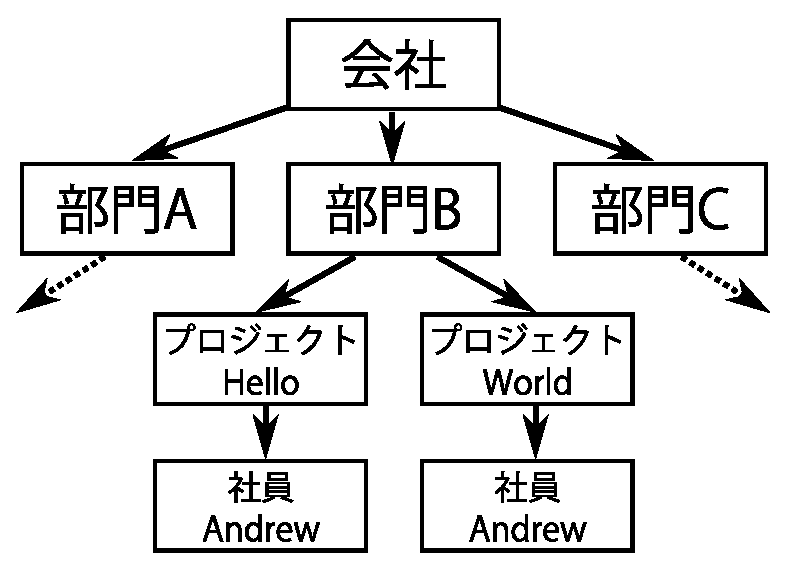
\includegraphics[width=5cm]{hayamiz/images/hierarchical-data-model.eps}
   \caption{階層型データモデル}
   \label{214539_12Jul12}
  \end{center}
 \end{minipage}
 \begin{minipage}{0.48\textwidth}
  \begin{center}
   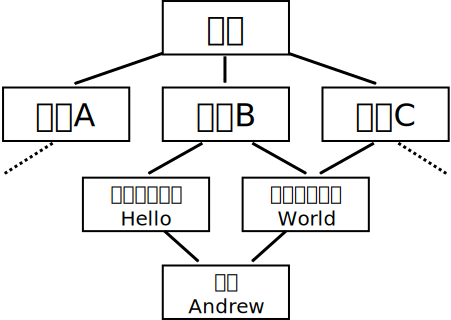
\includegraphics[width=5cm]{hayamiz/images/network-data-model.eps}
   \caption{ネットワーク型データモデル}
   \label{214707_12Jul12}
  \end{center}
 \end{minipage}
\end{figure}

階層型データモデルというのは、木構造を用いてデータを組織化したデータモデ
ルです。たとえば会社組織を階層型データモデルで表そうと思うと、会社の下に
は複数の部門が属しており、各部門の下には複数のプロジェクトがあり、各プロ
ジェクトの下には社員が属している、というようにスキーマを定義してゆきます
(図\ref{214539_12Jul12})。ここで、例えば2つのプロジェクトHelloとWorldに属
する1人の社員Andrewがいたとしたらどうでしょう。階層型データモデルでは、あ
るデータの実体(ここでは1人の社員)は親となるデータの実体(プロジェクト)
を複数持つことができません。そのため、各プロジェクトごとにAndrewのデータ
を持つことになり、データの重複が生じてしまいます。また、部門Bと部門Cが共
同でプロジェクトWorldを運営していることを表現しようと思うと、プロジェクト
のデータに加えてその下にぶら下がっている社員のデータも併せてコピーしなけ
ればなりません。このような欠点を克服したのがネットワーク型データモデルで
す(図\ref{214707_12Jul12})。ネットワーク型データモデルでは、データの実
体が複数の親を持つことができる有向グラフをデータ構造として採用したため、
前述のようなデータ重複の問題は発生しません。

ネットワーク型モデルによりより一般的なデータ構造を表現できるようにはなり
ました。しかし、階層型モデルやネットワーク型モデルに基づくデータベースは、
データのアクセスに一つ大きな問題を抱えていました。これらのデータベースに
おいてデータの問い合わせを行う際には、データの構造がどのようになっている
かを把握し、そしてどのような手順でデータを取得するかを利用者が知っている
必要があったのです。例えば図\ref{214707_12Jul12}のデータベースにおいて社
員Andrewのデータを取得するためには、「会社のデータを読みとり、部門Bのデー
タを読み取り、プロジェクトHelloのデータを読み取り、社員Andrewのデータを読
み取る」という手順を指定してあげなければなりません。このように、欲しいデー
タにアクセスするための``how'' をもって問い合わせを行うデータベースシステ
ムは、ユーザがデータの案内(navigation)をするという意味で{\bf ナビゲーショ
ナルデータベースシステム}と呼ばれます。

もしもナビゲーショナルデータベースシステムにおいて、図
\ref{214707_12Jul12}の会社で組織改変があり、各部門の下には課が設置され、
その下にプロジェクトが属するという構造にデータベースが修正されたとしたら
どうなるでしょう。これまで社員のデータにアクセスするアプリケーションは会
社→部門→プロジェクト→社員とたどっていましたが、会社→部門→課→プロジェ
クト→社員とたどるように修正しなければなりません。このように、ナビゲーショ
ナルデータベースシステムでは、ある特定のデータのみに興味があったとしても、
その上位構造に変化があった時にはデータにアクセスする方法を再構成しなけれ
ばなりませんでした。当時IBMはIMSという階層型データモデルにもとづくデータ
ベースシステムを開発していましたが、IMSを使ったシステムではデータ構造の変
更に伴うコードのメンテナンスにほとんどの時間を吸い取られていました。

歴史的には、階層型モデルはそのシンプルさ故に初期のデータベースシステムに
おいて採用され、その後により一般的なデータの組織化を行うことができるよう、
ネットワーク型モデルが発明されます。1969年にはCODASYLという委員会によって、
ネットワーク型データモデルの標準化が行われ、データベースシステムの情勢は
階層型モデルからネットワーク型モデルに移るかと思われました。

そこに登場したのが、1970年\footnote{正確にはリレーショナルデータモデルの
論文は1969年にIBMの社内技術報に掲載され、翌1970年に米国コンピュータ学会の
論文誌に掲載されます。}にCoddによって提唱されたリレーショナルデータモデル
です。リレーショナルデータモデルでは、データの論理的な構造と物理的な構造
が独立しているため、データ構造を変更するたびにアプリケーションを書き直す
必要がありません。また、ユーザは「どんなデータが欲しいか」を記述するたけ
で、具体的なアクセス方法はデータベース側が判断してデータを取得することが
できます。つまり、ナビゲーショナルデータベースシステムでは ``how'' を与え
なければデータのアクセスが行えなかったのですが、リレーショナルデータベー
スは ``what'' を与えるだけでデータのアクセスが可能となります\footnote{リ
レーショナルモデルの数学的な定義や、なぜそれにより``what''でデータの問い
合わせが可能となるのかの説明については、それだけで一冊の本になってしまう
ので他書に譲ります。}。

また、リレーショナルモデルは集合論にもとづくしっかりとした数学的基礎の上
に成り立っており、後のデータベースシステム研究の大きな基盤となりました。
これまでプログラマによるある種の職人芸の上に成り立っていたデータベースシ
ステムは、リレーショナルデータモデルの登場によって科学の領域へと押し上げ
られたのです。

ちなみに、データベースのお勉強をした人たちは、ドメイン、リレーション、タ
プル、主キー、外部キー、○○正規形という言葉に聞き覚えがあるかもしれませ
んが、これら教科書に載っているリレーショナルデータモデルのかなりの部分が
1970年の論文の段階で体系的にまとめられています。もちろん現在のリレーショ
ナルデータモデルは様々な改良が加えられていますが、その基本的な骨子はほぼ
そのままの形で残っています。この論文はタイトルで検索すればオンラインで読
むことができます。自分の勉強した知識と照らし合わせながら読んでみると面白
いのではないでしょうか。

\section{リレーショナルデータベースシステム黎明期}

\subsection{INGRESプロジェクト始動}

リレーショナルデータモデルがCoddによって提唱されてから3年が経った1973年が
終わろうとする頃、その論文が一人の若き研究者の目に留まりました。その人こ
そ、INGRESプロジェクト、そして後のデータベース業界全体を率いる存在となる
Michael Stonebraker です。1971年にミシガン大学で博士号を取得し、UC
Berkeleyで研究職についたばかりのStonebraker はテニュアトラック
\footnote{テニュアとは大学における終身雇用資格のことです。若手研究者は任
期の限られた研究職につき、テニュア獲得を目指して研究業績を積み上げてゆく、
というの米国における一般的な研究者のキャリアパスです。このテニュア獲得の
ための若手研究者が通る道をテニュアトラックと呼びます。テニュアトラックで
いかに論文を``量産''できる研究ネタを選ぶかというのは、若手研究者にとって
は人生に関わる重要な決断なのです。}を走り始めたばかりであり、何か良い研究
のネタはないかと思案していたところでした。そんな Stonebraker にとって、リ
レーショナルモデルは恰好の研究対象だったのでしょう\footnote{ちなみに
Stonebraker の博士論文は ``The Reduction of Large Scale Markov Models
for Random Chains'' というタイトルで、もともとは数学寄りの研究をしていた
ようです。 }。リレーショナルデータモデルに出会った Stonebraker は、
Eugene Wong と共にリレーショナルデータベースシステムの実装に乗り出します。
こうしてINGRESプロジェクトは始まりました。

% http://genealogy.math.ndsu.nodak.edu/id.php?id=31091

INGRESという名前は、{\bf IN}teractive {\bf G}raphic and {\bf RE}trieval
{\bf S}ystem の頭文字をとったもので、本来は UC Berkeley の経済学の研究チー
ムのために、地理情報をグラフィカルに表示するためのシステム研究として予算
を獲得していたプロジェクトでした。そこは本音と建前で、まずはデータを効率
的に取得するためのデータベースシステムが必要だ、ということで Stonebraker
達はデータベースシステムの開発にのめりこんでゆきます。

こうして走り始めたINGRESプロジェクトですが、データベースシステムを動かす
ためのコンピュータはありませんし、そもそも Stonebraker や Wong は大きなプ
ログラム開発の経験すらありませんでした。リレーショナルデータベースシステ
ムの先駆けであるINGRESは、まさにゼロからのスタートでした。

何はなくともデータベースシステムの開発環境がなければ話になりません。
INGRESプロジェクトが始まって Stonebraker が最初に取り組んだのは、コンピュー
タの調達と開発環境作りでした。当時といえば、データベースシステムを構築す
るためには高価なメインフレームを導入して、COBOLでプログラムを書くという時
代でした。リレーショナルデータベースシステムのように、まだ世の中に存在す
らしていないソフトウェアのために、研究職になりたての Stonebraker がメイン
フレームを手に入れることができるわけもありません。

そんな中、ミニコンピュータと呼ばれる、いわゆる現在のPCの先駆けとなる安価
なコンピュータシステムが1960年代に生まれ、そして1970年代にはミニコンピュー
タをビジネスに活用しようという動きが高まり、小型ビジネスコンピュータ市場
が生まれました。時を同じくして、ベル研究所では Ken Thompson 達によってミ
ニコンピュータ上で動作する汎用オペレーティングシステムUNIXの開発プロジェ
クトが始まりました。UNIXはもともとアセンブリで実装されていましたが、
Dennis Ritchie 達によってUNIX開発のためにC言語が開発され、1973年にはC言語
に移植されました。そう、まさにINGRESプロジェクトが始まったその年です。

Stonebraker は開発環境として UNIX を、そしてINGRESの実装言語としてC言語を
使うことを決めます。そして UNIX が動作するコンピュータとして選ばれたのが、
DECのPDP-11/70でした。UNIXが最初にベル研究所以外の場所でインストールされ
たのがこのINGRESプロジェクトであり、インストール時には Ken Thompson と
Dennis Ritchie が5MBのディスクを抱えてやってきたそうです。

\subsection{INGRESの進化}

INGRESプロジェクトでは、リレーショナルデータベースシステムの実装における
重要な技術が多数生み出されてゆきました。

\subsubsection{クエリ言語QUELとEQUEL}

リレーショナルデータベースでは、それ以前のナビゲーショナルデータベースと
は異なり、どんなデータが欲しいか``what''を記述するだけで、具体的にどのよ
うなデータ構造やアルゴリズムが実装されているかを一切知る必要なくデータを
取得することができる、というのが大きなウリの一つです。その``what''を記述
するための言語がクエリ言語です。皆さんのよく知っているSQLもクエリ言語の一
つです。

INGRESプロジェクトでは、クエリ言語としてQUELが開発されます。リレーショナ
ルデータモデルに併せて Codd はDSL/APLHAというクエリ言語を1971年に発表して
いるのですが、DSL/ALPHAは数学的な表記\footnote{DSL/ALPHAは関係演算
(relational calculus)をベースとして、量化子$\exists, \forall$や、論理演算
の記号$\lnot,\land,\lor$などがほぼそのまま用いられいていました}に基づいて
おりやや一般的にわかりやすいものではありませんでした。QUELはDSL/ALPHAをベー
スとして、数学的な表記のない``やさしい''クエリ言語として設計されました。

QUELがどんな言語なのか、簡単なサンプルコード\footnote{1975年のINGRESの論
文より引用}をみてみましょう。

\begin{center}
 \begin{minipage}{0.9\textwidth}
  \begin{verbatim}
RANGE OF C IS CITY
RETRIEVE INTO W(C.CNAME,
                DENSITY = C.POPULATION / C.AREA)
         WHERE C.STATE = 'California'
           AND C.POPULATION > 50000
  \end{verbatim}
 \end{minipage}
\end{center}

このサンプルコードでは、カリフォルニア州にある人口5万人以上の市について、
市の名前と人口密度の一覧を取得するという処理を行っています。一行目の
RANGE文では、処理の対象としてCITYテーブルを選択して、CITYテーブルのレコー
ドを表す変数名Cを宣言しています。二行目のRETRIEVE文は、SQLでいうところの
SELECT文に相当します。処理の結果は、一時テーブルとして作成されるWに保存さ
れます。細かい表記の違いを別にすると、現在使われているSQLとそれほど大きな
違いがないことがわかると思います。

\subsubsection{データ構造とアクセスメソッド}

\subsubsection{クエリ処理エンジン}

\subsection{System R}

INGRESプロジェクトからすこし遅れて、IBMでもリレーショナルデータベースシス
テム System R の研究開発が始まります。リレーショナルデータモデルの父であ
る Codd はIBMで働いていたにも関わらず、歴史を振り返るとIBMはリレーショナ
ルデータベースシステム開発において常に後塵を拝しています。

TODO:

\section{エピローグ}

1970年代には、Coddによるリレーショナルデータモデルの提唱に始まり、INGRES
やSystem Rの研究によってリレーショナルデータベースシステムが実用に耐えう
るものであることが証明されました。1981年には、Coddはその功績が認められ計
算機科学分野において最も権威ある賞であるチューリング賞を受賞します。

そして1970年代の終盤から1980年代は、商用リレーショナルデータベースシステ
ムが次々と登場し、熾烈な戦いを繰り広げてゆきます。

1977年、現在の Oracle の前身である Software Development Laboratories が
Larry Ellison と Robert Miner によって設立され、1979年にはSQLベースの商用
リレーショナルデータベースシステムとしては世界初となる Oracle RDBMS の発
売を開始します。

1979年、Jack Shemer、Philip Neches、Walter Muir、Jerold Modes、William
Worth、Carroll ReedによってTeradataが設立され、1984年には世界初の並列デー
タベースシステムDBC 1012をリリースします。

1980年、Lawrence Rowe、Michael Stonebraker、Eugene Wong、Gary
Morgenthaler によって INGRES 商用化のために Relational Technology (後の
Ingres Corp.)が設立され、翌1981年に最初の商用INGRESをリリースします。

時を同じくして、Roger Sippl と Laura King によって 1980年に Relational
Database Systems (後の Informix Software) が設立され、翌1981年に
Informix がリリースされます。

IBMは1981年にSQL/DSを、さらに1983年にはDB2をリリースしてリレーショナルデー
タベース市場に乗り出します。エンタープライズ市場の覇者であるIBMのこの動き
は、旧来のナビゲーショナルデータベースシステムに対する新興勢力リレーショ
ナルデータベースシステムの勝利を決定的なものにします。

1984年、Mark Hoffman、Bob Epstein、Jane Doughty、Tom Hagginによって
Sybaseが設立され、1986年にリレーショナルデータベースシステムSybaseをリリー
スします。後にSybaseはMicrosoftと提携してSybase SQL Serverを開発し、その
設計はMicrosoft SQL Serverにも受け継がれています。

同1984年、ミニコンピュータ市場を牽引するDECがOpenVMSオペレーティングシス
テムにおける機能として DEC Rdb を発表します。

1986年、無停止コンピュータシステムを主な事業として手がける Tandem
Computers が NonStop SQL をリリースします。

そして1990年代には更にプレイヤーが増えつつもその統廃合が進み、オブジェク
ト指向データベースシステムなど進行技術の登場、オープンソースのデータベー
スシステム隆盛の兆候など、データベースシステムは新たな時代へと突入してゆ
きます。

\section*{参考文献}

\small

\begin{itemize}
 \item E. F. Codd, ``A Relational Model of Data for Large Shared Data
       Banks'', {\it Communications of the ACM}, Volume 13, Number 6,
       1970
 \item E. F. Codd, ``A data base sublanguage founded on the relational
       calculus'', {\it Proceedings of the 1971 ACM SIGFIDET workshop
       on Data Description, Access and Control}, 1971
 \item C. J. Date, E. F. Codd, ``The relational and network approaches: Comparison of the
       application programming interfaces'', {\it Proceedings of the
       1974 ACM SIGFIDET workshop on Data Description, Access and
       Control}, 1975
 \item G. Held, M. Stonebraker, E. Wong, ``INGRES--A relational data
       base management system'', {\it Proceedings of AFIPS 1975 NCC},
       Volume 44, 1975
 \item M. Stonebraker, G. Held, E. Wong, P. Kreps, ``The design and
       implementation of INGRES'', {\it ACM Transactions on Database
       Systems}, Volume 1, Issue 3, 1976
 \item G. Held, M. Stonebraker, ``B-trees re-examined'', {\it Communications of the
       ACM}, Volume 21, Issue 2, 1978
 \item M. Stonebraker, ``Retrospection on a database system'', {\it ACM
       Transactions on Database Systems}, Volume 5, Issue 2, 1980
 \item D. Chamberlin, M. Astrahan, M. Blasgen, J. Gray, W. F. King,
       B. Lindsay, R. Lorie, J. Mehl, T. Price, F. Putzolu, P. Selinger,
       M. Schkolnick, D. Slutz, I. Traiger, B. Wade, R. Yost, ``A
       history and evaluation of System R'', {\it Communications of the
       ACM}, Volume 24, Issue 10, 1981
 \item M. Stonebraker, J. Woodfill, J. Ranstrom, M. Murphy, M. Meyer,
       E. Allman, ``Performance enhancements to a relational database
       system'', {\it ACM Transactions on Database Systems}, Volume 8,
       Issue 2, 1983
 \item Relational Technology Inc., ``INGRES The Distributed SQL
       Relational Database System Press Kit'', 1987
 \item National Research Council, ``Funding a Revolution: Government
       Support for Computing Research'', Natl Academy Pr, 1999
 \item M. Stonebraker, J. M. Hellerstein, ``What Goes Around Comes
       Around'', {\it Readings in Database Systems, Fourth Edition},
       Morgan Kaufmann, 2005
 \item A. Ances, ``RDBMS Workshop: Ingres and Sybase'', Computer
       History Museum, 2007
\end{itemize}

and so many online resources

\normalsize